\documentclass[12pt]{article}%

\usepackage{algorithm}%
\usepackage{algorithmic}%
\usepackage[utf8x]{inputenc}%
\usepackage[romanian]{babel}%
\usepackage{amssymb}%
\usepackage{natbib}%
\usepackage{amsmath} \usepackage{url}%
\usepackage{graphicx}%
\usepackage{color}

\hyphenation{Matlab}%
\hyphenation{Python}%
\hyphenation{Octave}%
\hyphenation{C}%

\definecolor{brightmaroon}{rgb}{0.76, 0.13, 0.28}
\newcommand{\mat}{{\color{brightmaroon} Matlab / Octave}}
\definecolor{cadmiumgreen}{rgb}{0.0, 0.42, 0.24}
\newcommand{\pyt}{{\color{cadmiumgreen} Python}}
\definecolor{cobalt}{rgb}{0.0, 0.28, 0.67}
\newcommand{\cc}{{\color{cobalt} C++}}

\usepackage{float} \floatname{algorithm}{Algoritmul}

\renewcommand{\algorithmicforall}{\textbf{pentru toate}}
\renewcommand{\algorithmicdo}{\textbf{execută}}
\renewcommand{\algorithmicuntil}{\textbf{până când}}
\renewcommand{\algorithmicend}{\textbf{termină}}
\renewcommand{\algorithmicif}{\textbf{dacă}}
\renewcommand{\algorithmicelse}{\textbf{altfel}}
\renewcommand{\algorithmicfor}{\textbf{ciclu}}
\renewcommand{\algorithmicthen}{\textbf{atunci}}
\renewcommand{\algorithmicrepeat}{\textbf{repetă}}
\renewcommand{\algorithmicendfor}{\algorithmicend\ \algorithmicfor}

\renewcommand{\algorithmicrequire}{\textbf{Intrări:}}
\renewcommand{\algorithmicensure}{\textbf{Ieșire:}}

\title{Învățare Automată - Laboratorul 9 \\ \textbf{Segmentarea și
    compresia imaginilor utilizând rețele Kohonen}}%
\author{Tudor Berariu \\ Laboratorul AIMAS \\
  Facultatea de Automatică și Calculatoare}%

\begin{document}
\maketitle%

\section{Scopul laboratorului}
\label{sec:son}

Scopul acestui laborator îl reprezintă înțelegerea și implementarea
unei rețele Kohonen. Aceasta va fi aplicată pentru rezolvarea unei
probleme de învățare nesupervizată: segmentarea
imaginilor. Implementarea se va realiza în \mat\footnote{este nevoie
  de pachetul \texttt{gnuplot-x11}}, \pyt\footnote{este nevoie de pachetele
  \texttt{python-matplotlib} și \texttt{imagemagick}} sau
\cc\footnote{este nevoie de biblitecile \texttt{libjpeg} și
  \texttt{libgtkmm}}.

\section{Rețele Kohonen}
\label{sec:train}

O rețea Kohonen este formată din $N$ neuroni dispuși liniar, sub forma
unei matrice sau, mai rar, în spații de dimensiuni mai mari. Această
așezare permite identificarea vecinătații unui neuron, concept
important în procesul de învățare. Scopul acestui tip de rețele este
ca neuronii \emph{învecinați} (apropiați) să răspundă unor semnale
similare, iar perechi de neuroni mai \emph{îndepărtați} să
caracterizeze exemple mai puțin asemănătoare.

Antrenarea rețelei Kohonen corespunde unei segmentări a spațiului de
intrare într-un număr de regiuni egal cu numărul de neuroni din
rețea. Atunci când un exemplu dintr-o astfel de regiune este transmis
rețelei, neuronul corespunzător trebuie să prezinte nivelul de
excitare maxim.

Nivelul de excitare al unui neuron este invers proporțional cu
distanța euclidiană dintre ponderile sale și valorile exemplului dat
la intrare. Practic, se va activa neuronul cel mai apropiat de
semnalul de intrare.

Pentru antrenarea rețelei se folosește Algoritmul~\ref{alg:kohonen},
unde rata de învățare $\eta$ și vecinătatea $\phi$ sunt funcții ce
depind de timp (numărul iterației).

În Algoritmul~\ref{alg:kohonen}, $\mathbf{W}$ este o matrice de
dimensiune $n_1 \times n_2 \times \ldots \times n_k \times d$ unde
$n_1, n_2, \ldots, n_k$ sunt dimensiunile laticei de neuroni ($n_1
\cdot n_2 \cdot \ldots \cdot n_k = N$), iar $d$ este dimensiunea
spațiului de intrare.

\begin{algorithm}
  \caption{Antrenarea Rețelelor Kohonen}
  \begin{algorithmic}[1]
    \REQUIRE spațiul de intrare $\mathbf{X}$, funcțiile $\eta$ (rata
    de învățare), $\phi$ (vecinătate) \ENSURE ponderile $\mathbf{W}$
    \STATE $\mathbf{W} \longleftarrow random (0,1)$ \STATE $t
    \longleftarrow 1$ \REPEAT \STATE se alege $\mathbf{x_i} \in
    \mathbf{X}$ aleator \STATE $w_z \longleftarrow
    \underset{\mathbf{w} \in \mathbf{W}}{\operatorname{argmin}}$
    $Distance(\mathbf{w},\mathbf{x_i})$

    \FORALL{$\mathbf{w_j} \in \mathbf{W}$} \STATE $\mathbf{w_j}
    \longleftarrow \mathbf{w_j} + \eta(t)
    \phi(w_z,t)(\mathbf{x_i}-\mathbf{w_j})$
    \ENDFOR
    \STATE $t \longleftarrow t + 1$ \UNTIL{algoritmul converge sau
      numărul maxim de iterații a fost atins}
  \end{algorithmic}
  \label{alg:kohonen}
\end{algorithm}


\section{Segmentarea imaginilor}
\label{sec:tasks}

Pentru a rezolva sarcinile de laborator alegeți unul din următoarele
limbaje de programare: \mat, \pyt{ }sau \cc. Puteți implementa de la
zero într-un alt limbaj la alegere, dar nu se recomandă acest lucru.

\subsection{Cerința 1, de încălzire: Negativul unei imagini}
\label{sec:task1}

\subsubsection*{\mat}
\label{sec:mat1}

În arhiva laboratorului se găsește fișierul
\texttt{negative.m}. Completați codul modificând valorile matricei
\texttt{neg\_pixels} din funcția \texttt{negative} pentru a calcula
negativul imaginii date la intrare.

Pentru a verifica dacă totul funcționează bine, rulați în \mat{ }următoarea comandă:
\begin{verbatim}
>> negative('imgs/1.jpg')
\end{verbatim}

Dacă ați implementat corect, pe ecran va apărea imaginea din
Figura~\ref{fig:neg}.

\subsubsection*{\pyt}
\label{sec:pyt1}

În arhiva laboratorului se găsește fișierul
\texttt{negative.py}. Completați codul modificând valorile listei
\texttt{neg\_pixels} din funcția \texttt{negative} pentru a calcula
negativul imaginii date la intrare.

Pentru a verifica dacă totul funcționează bine, executați în consolă:

\begin{verbatim}
 # chmod +x negative.py
 # ./negative.py imgs/1.jpg
\end{verbatim}

Dacă ați implementat corect, pe ecran va apărea imaginea din
Figura~\ref{fig:neg}.

\subsubsection*{\cc}

În arhiva laboratorului se găsește fișierul
\texttt{negative.cc}. Completați codul pentru a calcula negativul
imaginii date la intrare.

Pentru a verifica dacă implementarea este corectă, compilați și rulați
\texttt{./negative imgs/1.jpg}.

\begin{verbatim}
$ make clean
$ make negative
$ ./negative imgs/1.jpg
\end{verbatim}

Dacă ați implementat corect, pe ecran va apărea imaginea din
Figura~\ref{fig:neg}.

\begin{figure}[h]
  \centering
  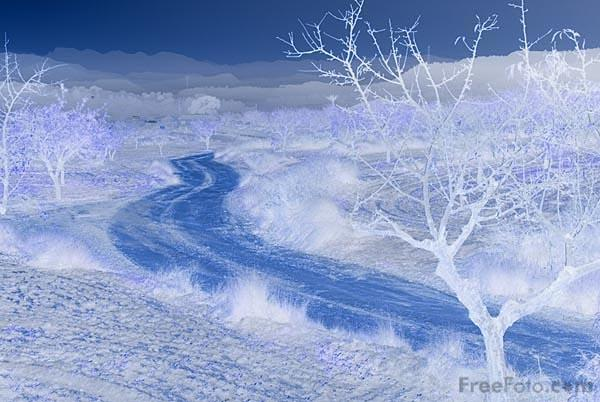
\includegraphics[width=0.75\textwidth]{src/imgs/1_neg.jpg}
  \caption{Negativul imaginii \texttt{1.jpg}}
  \label{fig:neg}
\end{figure}

\subsection{Taskul 2: Rata de învățare}
\label{sec:task2}

În al doilea pas trebuie să calculați rata de învățare. Pentru
început, implementați o descreștere liniară a ratei de învățare de la
$0.75$ la $0.1$.

După ce terminați toate task-urile, puteți încerca alte limite
(superioară și inferioară) pentru rata de învățare, precum și variații
pătratice, exponențiale, etc. pentru a vedea cum influențează
rezultatul segmentării.


\subsubsection*{\mat}
\label{mat2}

Deschideți fișierul \texttt{learning\_rate.m} și modificați corpul
funcției \texttt{learning\_rate} astfel încât să întoarcă valoarea
ratei de învățare în funcție de numărul iterației curente și numărul
total de iterații.

Pentru o verificare rapidă a codului rulați în \mat:
\begin{verbatim}
>> plot_learning_rate
\end{verbatim}

\subsubsection*{\pyt}
\label{pyt2}

Deschideți fișierul \texttt{learning\_rate.py} și modificați corpul
funcției \texttt{learning\_rate} astfel încât să întoarcă valoarea
ratei de învățare în funcție de numărul iterației curente și numărul
total de iterații.

Pentur o verificare rapidă a codului, rulați în Python:
\begin{verbatim}
 # chmod +x plot_learning_rate.py
 # ./plot_learning_rate.py
\end{verbatim}

\subsubsection*{\cc}
\label{cc2}

Implementați funcția \texttt{double learning\_rate(int, int)} din
fișierul \texttt{learning\_rate.cc}  astfel încât să întoarcă valoarea ratei de
învățare în funcție de numărul iterației curente și numărul total de
iterații.

\begin{verbatim}
make clean
make print_learning_rate
./print_learning_rate | gnuplot -e "plot '-' with lines" --persist
\end{verbatim}

\subsection{Exercițiul 3: Raza vecinătății}
\label{sec:task3}

În cadrul exercițiului 3 trebuie să modificați funcția \texttt{radius}
astfel încât să întoarcă valoarea razei vecinătății în funcție de
numărul iterației, dar și de dimensiunile rețelei Kohonen.

Pentru început, implementați o descreștere liniară a razei vecinătății
de la $\frac{\max(width,height)}{2}$ către valoarea 0 (vecinătatea
unui neuron nu conține alți neuroni în afară de acesta).

După ce implementați tot algoritmul încercați valori de start mai mici
pentru rază și descreșteri mai rapide și observați cum variază
rezultatele.

\subsubsection*{\mat}
\label{mat3}

În arhivă se găsește fișierul \texttt{radius.m}. Completați aici
implementarea funcției \texttt{radius}. Pentru a verifica rezolvarea,
rulați în \mat:
\begin{verbatim}
>> plot_radius
\end{verbatim}

\subsubsection{\pyt}
\label{sec:pyt3}

Între sursele \pyt găsiți fișierul \texttt{radius.py}. Modificați
corpul funcției astfel încât să calculeze rata vecinătății conform
indicațiilor de mai sus. Pentru verificare executați:

\begin{verbatim}
 $ chmod +x plot_radius.py
 $ ./plot_radius.py
\end{verbatim}

\subsubsection{\cc}
\label{sec:cc3}

În fișierul \texttt{radius.cc} completați codul funcției
\texttt{double radius(int iter\_no, int iter\_count, int height, int
  width)} astfel încât să calculeze raza vecinătății conform
indicațiilor de mai sus. Verificați-vă astfel:

\begin{verbatim}
 $ make clean
 $ make print_radius
 $ ./print_radius | gnuplot -e "plot '-' with lines" --persist
\end{verbatim}

\subsection{Exercițiul 4: Vecinătatea}
\label{sec:task4}

Vecinătatea reprezintă mulțimea acelor neuroni ale căror ponderi vor
fi actualizate într-un ciclu. Mulțimea cuprinde neuronul
\emph{câștigător} și neuronii aflați la o distanță mai mică decât raza
vecinătății (vezi taskul 3).

Modificați funcția \texttt{neighbourhood(y, x, radius, height, width)}
astfel încât să întoarcă o matrice de dimensiunea rețelei Kohonen care
să aibă valoarea 1 pentru neuronii din interiorul vecinătății și zero
pentru ceilalți.

Parametrii funcției sunt:
\begin{itemize}
\item \texttt{y} - coordonata y (linia) a neuronului câștigător
  (centrul vecinătății)
\item \texttt{x} - coordonata x (coloana) a neuronului câștigător
  (centrul vecinătății)
\item \texttt{radius} - valoarea razei
\item \texttt{height} - înălțimtea laticei (bidimensionale) de neuroni
\item \texttt{width} - lățimea laticei (bidimensionale) de neuroni
\end{itemize}

După terminarea tuturor exercițiilor, vă puteți întoarce la funcția
neighbourhood pentru a experimenta cu valori zecimale din intervalul
$[0,1]$ (1 în centru și valori ce descresc pe măsură ce distanța față
de centru crește).

\subsubsection*{\mat}
\label{sec:mat4}

Deschideți fișierul \texttt{neighbourhood.m} și implementați funcția
urmând indicațiile date.

Pentru verificare, introduceți în {\color{red} Matlab / Octave}:
\begin{verbatim}
octave:1> neighbourhood(4,4,3,7,7)
ans =

   0   0   0   1   0   0   0
   0   1   1   1   1   1   0
   0   1   1   1   1   1   0
   1   1   1   1   1   1   1
   0   1   1   1   1   1   0
   0   1   1   1   1   1   0
   0   0   0   1   0   0   0

octave:2> neighbourhood(6,5,3,7,7)
ans =

   0   0   0   0   0   0   0
   0   0   0   0   0   0   0
   0   0   0   0   1   0   0
   0   0   1   1   1   1   1
   0   0   1   1   1   1   1
   0   1   1   1   1   1   1
   0   0   1   1   1   1   1
\end{verbatim}


\subsubsection*{\pyt}
\label{sec:pyt4}

Implementați funcția în fișierul \texttt{neighbourhood.py} și testați
astfel:
\begin{verbatim}
 $ chmod +x neighbourhood.py
 $ ./neighbourhood.py 4 4 3 7 7
[[0, 0, 0, 1, 0, 0, 0],
 [0, 1, 1, 1, 1, 1, 0],
 [0, 1, 1, 1, 1, 1, 0],
 [1, 1, 1, 1, 1, 1, 1],
 [0, 1, 1, 1, 1, 1, 0],
 [0, 1, 1, 1, 1, 1, 0],
 [0, 0, 0, 1, 0, 0, 0]]
 $ ./neighbourhood.py 6 5 3 7 7
[[0, 0, 0, 0, 0, 0, 0],
 [0, 0, 0, 0, 0, 0, 0],
 [0, 0, 0, 0, 1, 0, 0],
 [0, 0, 1, 1, 1, 1, 1],
 [0, 0, 1, 1, 1, 1, 1],
 [0, 1, 1, 1, 1, 1, 1],
 [0, 0, 1, 1, 1, 1, 1]]
\end{verbatim}

\subsubsection*{\cc}
\label{sec:cc4}

Implementați funcția în fișierul \texttt{neighbourhood.cc}. Pentru a
vă testa implementarea:
\begin{verbatim}
$ make clean
$ make print_neighbourhood
$ ./print_neighbourhood 4 4 3 7 7
0 0 0 1 0 0 0
0 1 1 1 1 1 0
0 1 1 1 1 1 0
1 1 1 1 1 1 1
0 1 1 1 1 1 0
0 1 1 1 1 1 0
0 0 0 1 0 0 0
$ ./print_neighbourhood 6 5 3 7 7
0 0 0 0 0 0 0
0 0 0 0 0 0 0
0 0 0 0 1 0 0
0 0 1 1 1 1 1
0 0 1 1 1 1 1
0 1 1 1 1 1 1
0 0 1 1 1 1 1
\end{verbatim}

\subsection{Taskul 5: Antrenarea rețelei Kohonen}
\label{sec:task5}

Completați corpul funcției \texttt{som\_segmentation} pentru a calcula
ponderile neuronilor conform Algoritmului~\ref{alg:kohonen}. Folosiți
funcțiile implementate anterior. Parametrul $n$ reprezintă lungimea
matricei pătratice de neuroni ($N = n^2$).

$\mathbf{W}$ este o matrice de dimensiune $n \times n \times 3$, adică
va conține $n^2$ valori RGB.

Implementarea se va face în fișierul \texttt{som\_segmentation.m} dacă lucrați în
\mat, în fișierul \texttt{som\_segmentation.py} dacă lucrați în \pyt sau în fișierul \texttt{som\_segmentation.cc} dacă alegeți \cc.

\subsection{Taskul 6: Segmentarea imaginii}
\label{sec:task6}

Completați funcția \texttt{som\_segmentation} pentru a
construi o imagine modificată pornind de la cea originală și înlocuind
fiecare pixel cu valorile neuronului cel mai apropiat (distanță
euclidiană; după antrenarea rețelei).

În final, imaginea nouă (\texttt{seg\_pixels}) trebuie să conțină doar
valori egale cu ponderile neuronilor din rețeaua antrenată.

Salvați imaginea pe disc adăugând la numele fișierului original
sufixul \texttt{\_seg} (de exemplu \texttt{1\_seg.jpg}).

Un posibil rezultat folosind o rețea cu 9 neuroni este în
Figura~\ref{fig:seg}.

\begin{figure}[h]
  \centering
  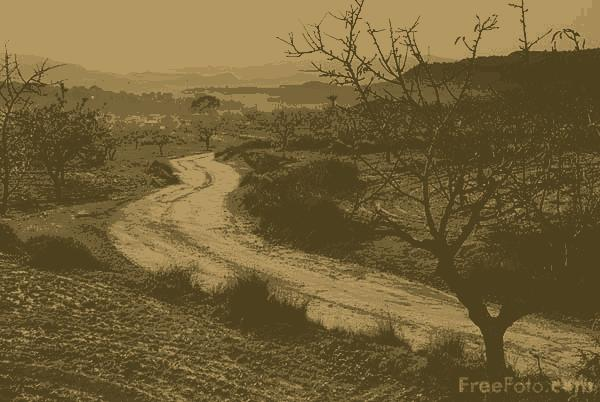
\includegraphics[width=0.75\textwidth]{src/imgs/1_seg.jpg}
  \caption{O posibilă segmentare a imaginii \texttt{1.jpg}}
  \label{fig:seg}
\end{figure}

\subsubsection*{\mat}
\label{sec:mat6}

Rezolvarea se va face, la fel ca la Exercițiul 5, în fișierul
\texttt{som\_segmentation.m}. Rulați apoi:
\begin{verbatim}
> som_segmentaion('imgs/3.jpg', 4)
\end{verbatim}

\subsubsection*{\pyt}
\label{sec:py6}

Rezolvarea se va face, la fel ca la Exercițiul 5, în fișierul
\texttt{som\_segmentation.py}. Rulați apoi:
\begin{verbatim}
$ ./som_segmentation imgs/3.jpg 4
\end{verbatim}

\subsubsection*{\cc}
\label{sec:cc6}

Rezolvarea se va face, la fel ca la Exercițiul 5, în fișierul
\texttt{som\_segmentation.cc}. Rulați apoi:
\begin{verbatim}
$ make clean
$ make som_segmentation
$ ./som_segmentation imgs/3.jpg 4
\end{verbatim}

\end{document}